\documentclass[11pt]{article}
\usepackage[margin=1in]{geometry}
\usepackage{amsmath,amssymb,bm}
\usepackage{graphicx}
\usepackage{booktabs}
\usepackage{caption}
\usepackage[table]{xcolor}
\usepackage{hyperref}
\hypersetup{colorlinks=true,linkcolor=blue!50!black,citecolor=blue!50!black}
\graphicspath{{figs/}}
\captionsetup{font=small}
\newcommand{\Rd}{\mathbb{R}}
\title{\textbf{Covert spatial cueing in a recurrent vision transformer:\\
frame-gated attention, cued change-detection, and the dynamics of a learned change-lock}}
\author{Recurrent Vision Transformer Project --- single-variant analysis}
\date{Model checkpoint: conv front-end $+$ cross-attention $+$ JEPA, iteration 9{,}599}

\begin{document}
\maketitle

\begin{abstract}
\noindent We analyse a recurrent vision transformer that learns covert visual attention purely from
sparse reward on a cued orientation--change-detection task. The agent comprises a learned convolutional
front-end (a small squeeze-and-excitation residual network), a single-head \emph{cross-attention}
recurrent transformer whose keys and values span both the current image and a recurrent memory, a
per-patch spatial xLSTM, and a distributional actor--critic, trained end-to-end with reinforcement
learning and an auxiliary temporal self-distillation (JEPA) objective. The trained agent solves the
task at $\approx\!0.87$ correct. Dissecting its attention reveals a strikingly legible algorithm. (i)
The cross-attention is \emph{frame-gated}: it reads the image essentially only on the cue frame and
operates from memory on every other frame. (ii) The cue-frame read is spatially precise: the
non-cued query patches place $\approx\!1.0$ of their attention on the cued image patch. (iii) Change
detection produces a memory \emph{change-lock} whose timing is cue-dependent: validly cued changes are
attended one frame earlier than invalidly cued changes --- an attentional cueing benefit. (iv) The
allocation of attention is invariant to cue validity (ring completeness) and cue value (colour);
these variables instead shape the decision, yielding a behavioural cueing benefit (validly cued changes
are detected at lower magnitude than invalidly cued changes) without modulating the attention maps.
We give the explicit attention computation, a complete battery of raw attention maps across cue
position, validity, value, and change conditions, psychometric functions over change magnitude,
temporal decoding of task variables from the recurrent state, and a causal perturbation of the memory
read. The model reproduces hallmark signatures of primate covert spatial attention.
\end{abstract}

\section{Introduction}
Covert spatial attention---the selective prioritisation of a location without an eye movement---is a
central construct in primate vision. A cue indicates where a behaviourally relevant event is likely to
occur; valid cues speed and sensitise detection at the cued location, invalid cues impair it, and the
size of this cueing benefit scales with cue reliability and stimulus value. We ask whether an agent that
must \emph{learn} a cued change-detection task from reward alone develops an internal attentional
algorithm with these signatures, and if so, what that algorithm is mechanistically. We study a single
trained checkpoint of a recurrent vision transformer and report (a) its behaviour, (b) the dynamics of
its learned attention, and (c) the causal role of its memory read. Throughout we distinguish the
\emph{current image} (what the model can see now) from the \emph{recurrent memory} (what it has
integrated), because the model's algorithm is precisely a scheduled hand-off between the two.

\section{Methods}
\subsection{Task}
Each trial is a $T=7$-frame sequence of $50\times50$ RGB frames partitioned row-major into four
$25\times25$ quadrants, indexed $\{S1{=}\text{TL},\,\text{TR},\,\text{BL},\,S4{=}\text{BR}\}$. The
timeline is: $t{=}0$ blank; $t{=}1$ \emph{cue}; $t{=}2$ blank; $t{=}3$--$6$ four oriented Gabor
stimuli (one per quadrant), with independent orientation noise each frame. On half of trials, at the
change time $t{=}5$ exactly one Gabor's orientation steps by $\Delta\theta$. The cue is a coloured disc
marking one quadrant; its \emph{colour} signals value ($\text{red}{=}5$, $\text{green}{=}3$,
$\text{blue}{=}1$) and its \emph{ring completeness} (proportion $p\in\{0.25,0.5,0.75,1.0\}$) signals
validity (the probability that a change, if it occurs, is at the cued quadrant). The agent emits one of
two actions each frame, \texttt{wait} or \texttt{declare-change}; declaring at or after the change time
on a change trial is rewarded (value-weighted), as is waiting through a no-change trial (correct
rejection). Declaring early or on a no-change trial is a false alarm. ``Correct'' denotes any rewarded
trial.

\subsection{Architecture}
\textbf{Convolutional front-end.} Each quadrant patch $o_i\in\Rd^{25\times25\times3}$ is encoded by a
shared small SE-ResNet $f_\theta$: a $3\times3$ stem followed by three squeeze-and-excitation residual
stages (GroupNorm, SiLU, channel-attention, progressive downsampling $32\!\to\!64\!\to\!128$), global
average pooling, and an output normalisation, giving $\hat o_i = f_\theta(o_i)\in\Rd^{128}$
($\sim\!0.59$M shared parameters; trained end-to-end, no pretraining). The token for patch $i$ at time
$t$ is
\begin{equation}
\bm{x}_i^{(t)} = \big[\,\hat o_i^{(t)} \;\Vert\; \bm{\rho}_i \;\Vert\; \bm{\tau}^{(t)}\,\big]\in\Rd^{140},
\qquad X^{(t)}=\big(\bm x_1^{(t)},\dots,\bm x_4^{(t)}\big)^{\!\top}\in\Rd^{4\times140},
\end{equation}
where $\bm\rho_i\in\Rd^4$ is a one-hot patch-position code and $\bm\tau^{(t)}\in\Rd^8$ a one-hot
timestep code.

\textbf{Cross-attention recurrent transformer.} Let $H^{(t-1)}\in\Rd^{4\times128}$ be the previous
recurrent memory (the xLSTM cell, one $128$-vector per patch). The transformer block forms queries from
the image and keys/values from \emph{both} the image and the memory:
\begin{align}
Q &= X^{(t)}W_q \in\Rd^{4\times140}, \\
K &= \big[\,X^{(t)}W_{kx}\;\Vert\;H^{(t-1)}W_{kh}\,\big]\in\Rd^{8\times140}, \qquad
V = \big[\,X^{(t)}W_{vx}\;\Vert\;H^{(t-1)}W_{vh}\,\big]\in\Rd^{8\times140}.
\end{align}
The $8$ keys are ordered so that $j\in\{0,1,2,3\}$ are the four \emph{image} patches and
$j\in\{4,5,6,7\}$ are the four \emph{memory} tokens (memory token $j{-}4$ is the per-patch xLSTM cell of
quadrant $j{-}4$). The attention matrix is
\begin{equation}
\boxed{\;A^{(t)} = \mathrm{softmax}_{\,\mathrm{keys}}\!\left(\frac{Q K^{\top}}{\sqrt{140}}\right)\in\Rd^{4\times8},
\qquad \sum_{j=0}^{7} A^{(t)}_{ij}=1\ \ \forall i,\;}
\label{eq:attn}
\end{equation}
so $A^{(t)}_{ij}$ is the weight that query patch $i$ places on key $j$; the first four columns are the
\emph{image-key} map and the last four the \emph{memory-key} map. The block output is the
residual update $Z^{(t)} = X^{(t)} + A^{(t)}V$. Crucially, the current image enters $Z$ through the
residual $X^{(t)}$ regardless of $A^{(t)}$, so suppressing image-key \emph{attention} does not blind the
model to the current frame.

\textbf{Recurrent cell.} $Z^{(t)}$ drives a per-patch spatial xLSTM with exponential input/forget gates,
$(\,\tilde I,\tilde F,\tilde O,\tilde U) = W Z^{(t)} + R H^{(t-1)}$, stabiliser
$M=\max(\tilde F+M^{-},\tilde I)$, $I=e^{\tilde I-M}$, $F=e^{\tilde F+M^{-}-M}$,
$C^{(t)}=F\odot C^{(t-1)}+I\odot\tanh \tilde U$, $N^{(t)}=F\odot N^{(t-1)}+I$,
$H^{(t)}=\sigma(\tilde O)\odot C^{(t)}/N^{(t)}$, with $H^{(t)}\in\Rd^{4\times128}$. The flattened cell
$\mathrm{vec}(H^{(t)})\in\Rd^{512}$ feeds a 3-layer ELU actor (policy over the two actions) and a
quantile-regression distributional critic.

\textbf{Training.} The agent is trained by a distributional actor--critic (MPO-style policy improvement
$+$ QR-DQN critic, prioritised replay, EMA target) on reward alone, with an auxiliary V-JEPA temporal
self-distillation loss on the cell output (an EMA teacher; structured $4\times256$ prototype softmaxes;
coefficient $0.5$). The front-end out-normalisation is LayerNorm in this checkpoint; we verify the
analysis loads the exact trained architecture (zero missing / unexpected parameters).

\subsection{Analysis}
All attention quantities are the mean of $A^{(t)}$ over $B{=}96$ trials per condition; we report the raw
softmax weights of Eq.~\eqref{eq:attn} with \emph{no} further normalisation. We treat the four rows of
$A^{(t)}$ (the four query patches) separately wherever it matters: query-averaging dilutes the
spatially-localised cue read (the per-query value $\approx\!1.0$ becomes $\approx\!0.75$ once the cued
query, which reads $\approx\!0$ on its own patch, is included), so cue-frame statistics are reported for the cued
query's own row. ``Change-lock'' is quantified as the excess of the changed quadrant's memory-key weight
over the uniform value $1/4$, per query. To control cue--change confounds we always run the dissociation
\emph{both ways} (cue@S1/change@S4 \emph{and} cue@S4/change@S1). Psychometric functions are
$P(\text{declare}\ge t_{\text{chg}})$ over $B{=}160$ episodes per point; the greedy press time is read
open-loop from forced-wait rollouts, which is exact for the first press because the observations up to
the press do not depend on it. Decoding uses
4-fold cross-validated logistic regression on $\mathrm{vec}(H^{(t)})$. Causal perturbations additively
bias selected key logits before the softmax in Eq.~\eqref{eq:attn} during the Gabor phase.

\section{Results}
\subsection{Behaviour: a covert-cueing psychometric signature}
On natural trials (env-drawn cue, value, validity, and change; $N{=}600$) the agent is correct on
$0.865$ of trials---hit rate $0.76$ on change trials, correct-rejection $0.96$ on no-change trials,
false-alarm rate $0.044$, with presses clustered on the change frame (RT $5.1\pm0.3$). It is thus a
conservative detector (high correct-rejection, a fraction of changes missed). Under forced conditions,
detection increases with change magnitude, saturating by $44^\circ$ (Fig.~\ref{fig:psy}). Crucially,
validly cued changes (change at the cued quadrant) are detected at \emph{lower} magnitude than
invalidly cued changes: $P(\text{detect})$ at $|\Delta\theta|=16^\circ$ is $0.58$ (valid) vs.\ $0.43$
(invalid), and at $28^\circ$ is $0.99$ vs.\ $0.94$; both saturate by $44^\circ$ and both floor near the
false-alarm rate (the forced no-change rate is $0.075$) at $0^\circ$. This left-shift of the valid
psychometric function is the classic covert-cueing benefit. The benefit is driven by the spatial cue,
not the displayed validity ring: holding magnitude at $28^\circ$, the valid/invalid gap is essentially
constant across displayed proportions $0.25$--$1.0$ (valid $0.975$--$1.0$, invalid $\approx0.93$--$0.95$;
Fig.~\ref{fig:valbeh}). Detection latency is $\approx\!5$ frames (presses cluster on the change frame)
for both validities.

\begin{figure}[t]\centering
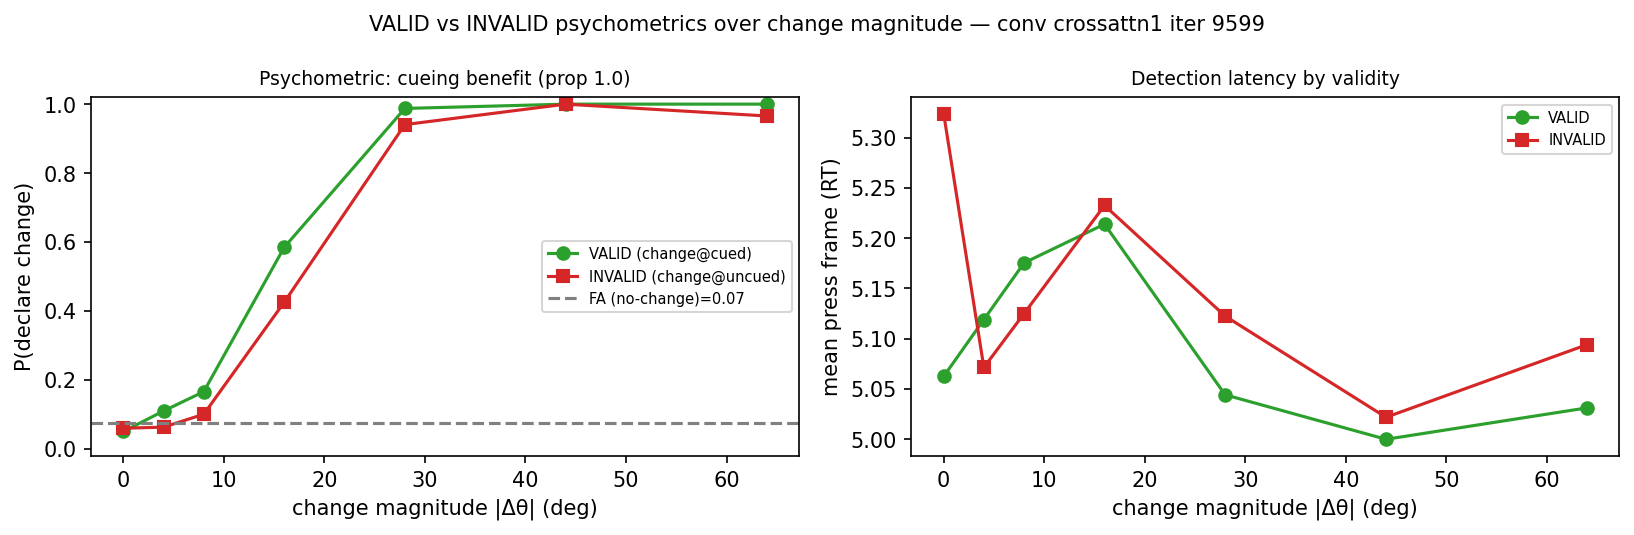
\includegraphics[width=\textwidth]{dd4_psychometric.png}
\caption{\textbf{Psychometric cueing benefit.} $P(\text{declare change}\ge t_{\text{chg}})$ vs.\ change
magnitude for validly (green) vs.\ invalidly (red) cued changes at proportion $1.0$, averaged over cue
position; dashed grey is the no-change false-alarm rate. Right: detection latency (press frame). Valid
detection is left-shifted (lower threshold); both saturate at high magnitude.}
\label{fig:psy}
\end{figure}

\subsection{Frame-gated attention: read the cue, then run from memory}
The cross-attention partitions the trial into a single image-reading frame and an otherwise
memory-driven trajectory (Fig.~\ref{fig:gate}). Summed image-key attention is near its ceiling on the
cue frame ($t{=}1$) and near zero on every Gabor frame; the complementary memory-key mass dominates the
accumulation and change frames. The current image is never \emph{lost} (it enters the cell through the
residual $X^{(t)}$), but the model chooses to \emph{attend} the image only when the cue is present.

\begin{figure}[t]\centering
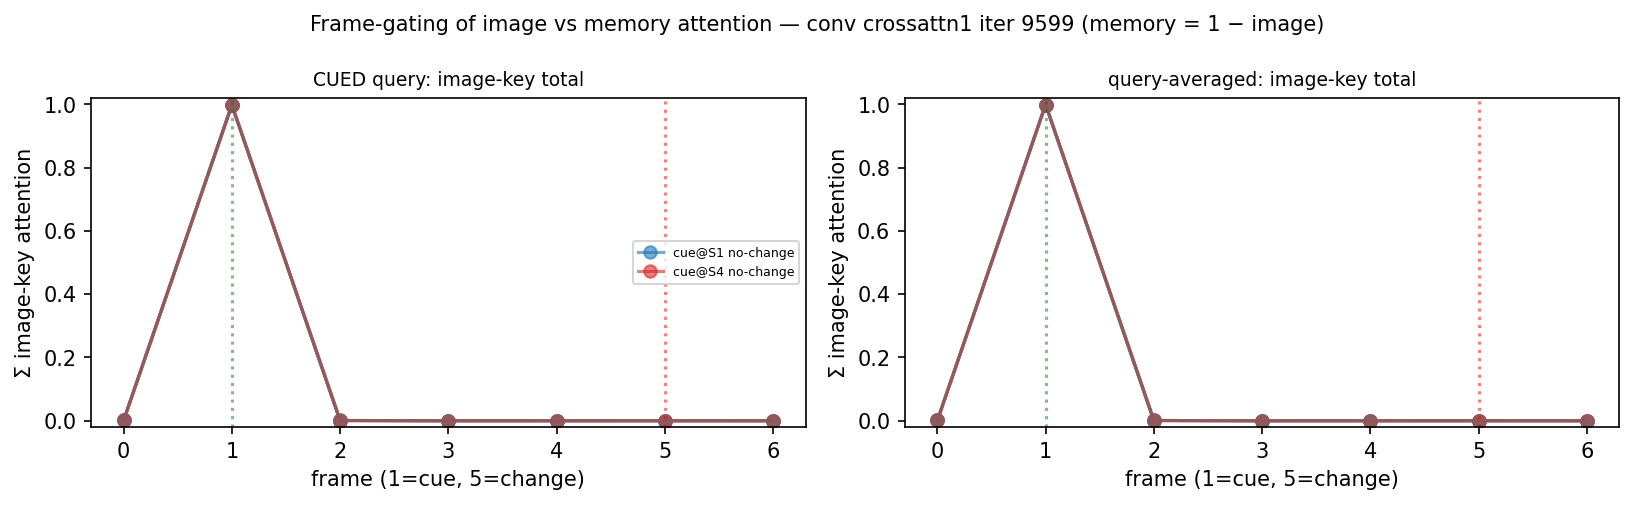
\includegraphics[width=\textwidth]{dd2_framegate.png}
\caption{\textbf{Frame-gating.} Summed image-key attention by frame for the cued query (left) and
averaged over queries (right), all six cue$\times$change conditions overlaid --- only the two no-change
conditions are labelled, as all six coincide through the cue read (memory $=1-$image). Image
attention spikes at the cue frame ($t{=}1$, dotted green) and collapses to near zero across the Gabor
and change frames (change at $t{=}5$, dotted red).}
\label{fig:gate}
\end{figure}

\subsection{The cue-frame read is spatially precise}
On the cue frame, the three non-cued query patches place $\approx\!1.00$ of their attention on the
\emph{cued} image patch, while the cued patch's own query reads the other quadrants (its self-weight is
$\approx\!0$); the cue is thereby broadcast to all four tokens. This is visible as the bright column at
the cued quadrant in the $t{=}1$ image-key maps of Fig.~\ref{fig:mapimg} and is identical across the
no-change, valid, and invalid conditions (the change has not yet occurred).

\begin{figure}[p]\centering
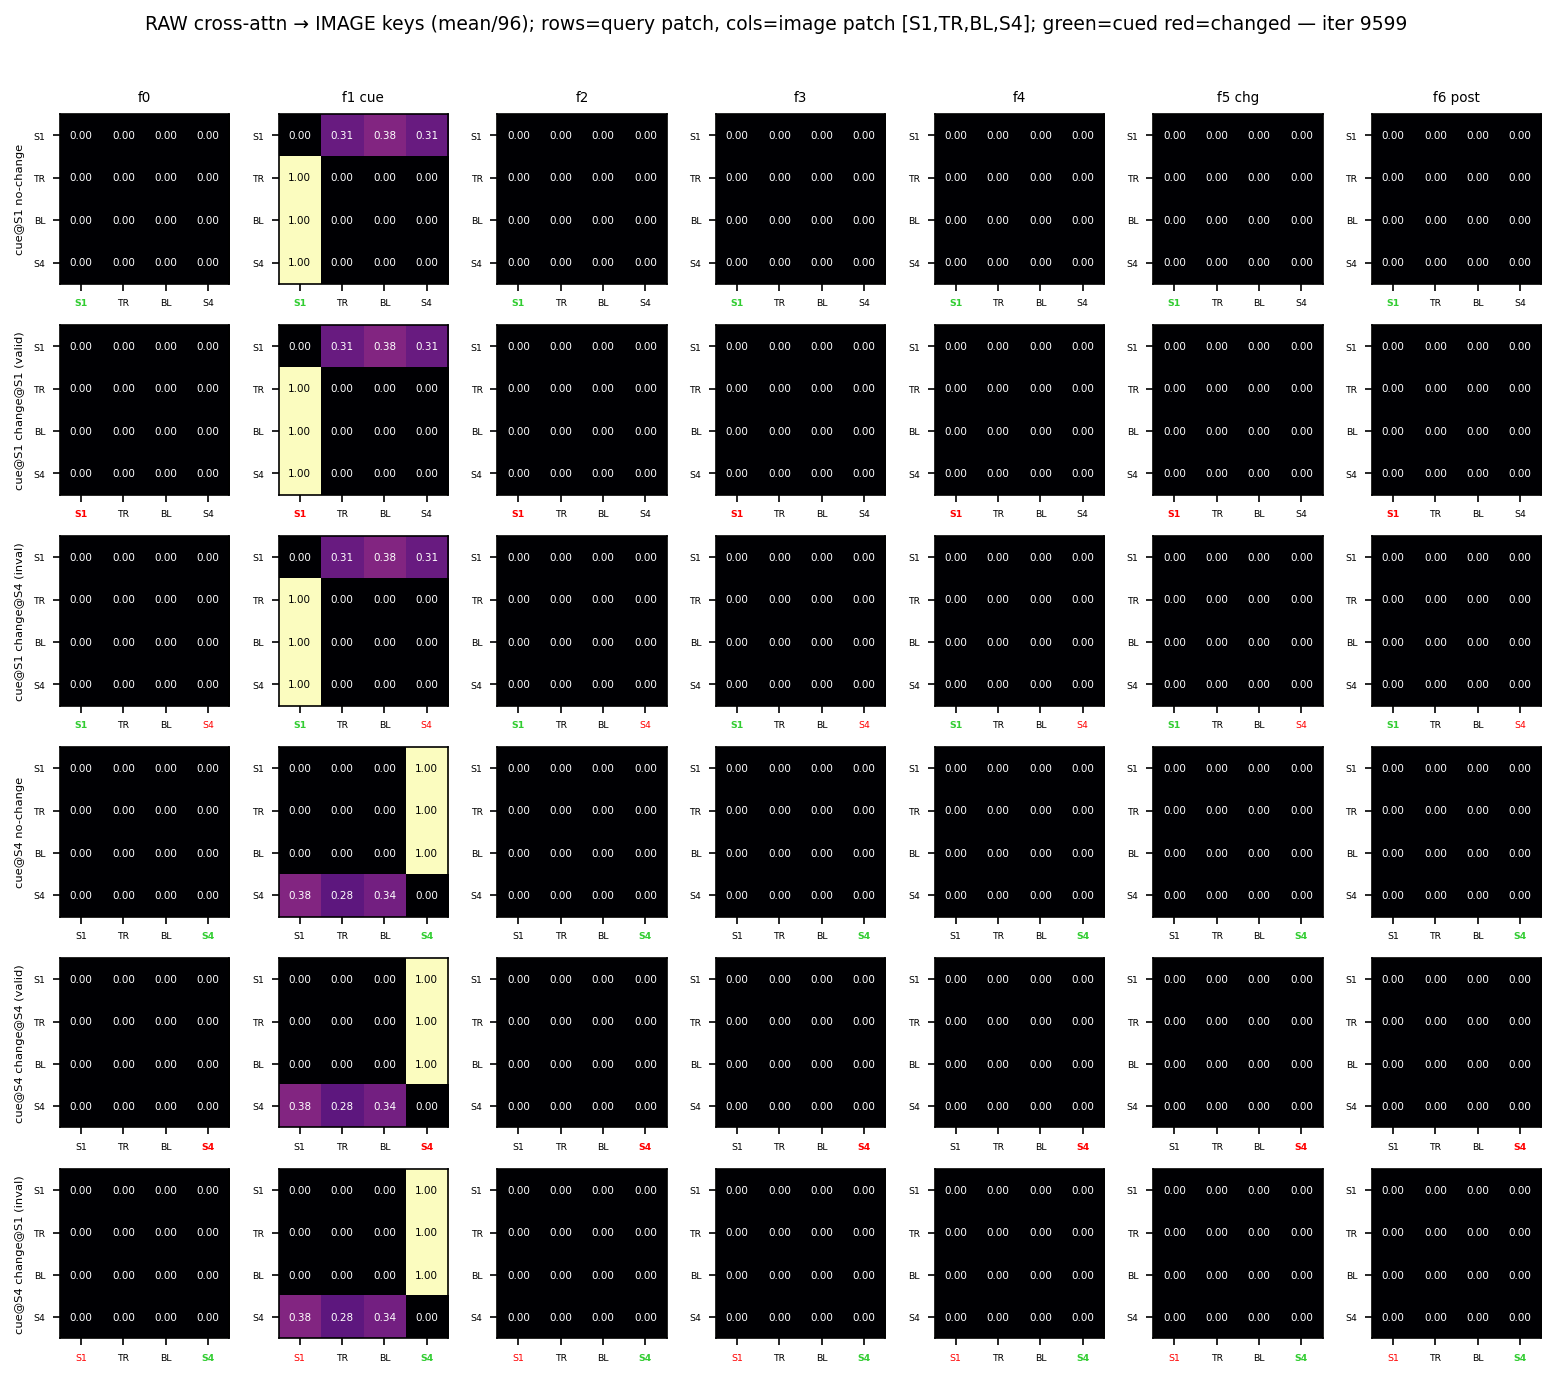
\includegraphics[width=\textwidth]{dd2_maps_image.png}
\caption{\textbf{Raw image-key attention maps}, mean over $96$ trials. Rows are the six
cue$\times$change conditions; columns are frames $t{=}0$--$6$. Within each $4\times4$ tile, rows are
query patches and columns are image patches $[S1,\text{TR},\text{BL},S4]$; the cued column is labelled
green, the changed column red. The cue frame ($t{=}1$) shows the sharp read of the cued patch; Gabor
frames are dark (image attention $\approx0$).}
\label{fig:mapimg}
\end{figure}

\subsection{A cue-timed memory change-lock}
After the cue, the memory read tracks the cued quadrant; when the change occurs, the memory read
re-points onto the \emph{changed} quadrant---but with a timing that depends on the cue
(Fig.~\ref{fig:mapmem}; quantified in Table~\ref{tab:lock}). For \emph{validly} cued changes (change at
the monitored, cued quadrant), the change-lock is already present on the change frame $t{=}5$ (excess
$+0.20$ on the changed memory token) and is strong one frame later ($+0.74$ at $t{=}6$). For
\emph{invalidly} cued changes (change at an unmonitored quadrant), there is \emph{no} lock on $t{=}5$
(the changed token is at or slightly below uniform, $-0.03$) and the lock appears only at $t{=}6$
($+0.70$). Thus the cue buys one frame of detection latency in the attention itself---the attentional
analogue of the behavioural cueing benefit. The lock is genuine and conditional: on no-change trials the
memory read stays on the cued quadrant and never re-points.

\begin{figure}[p]\centering
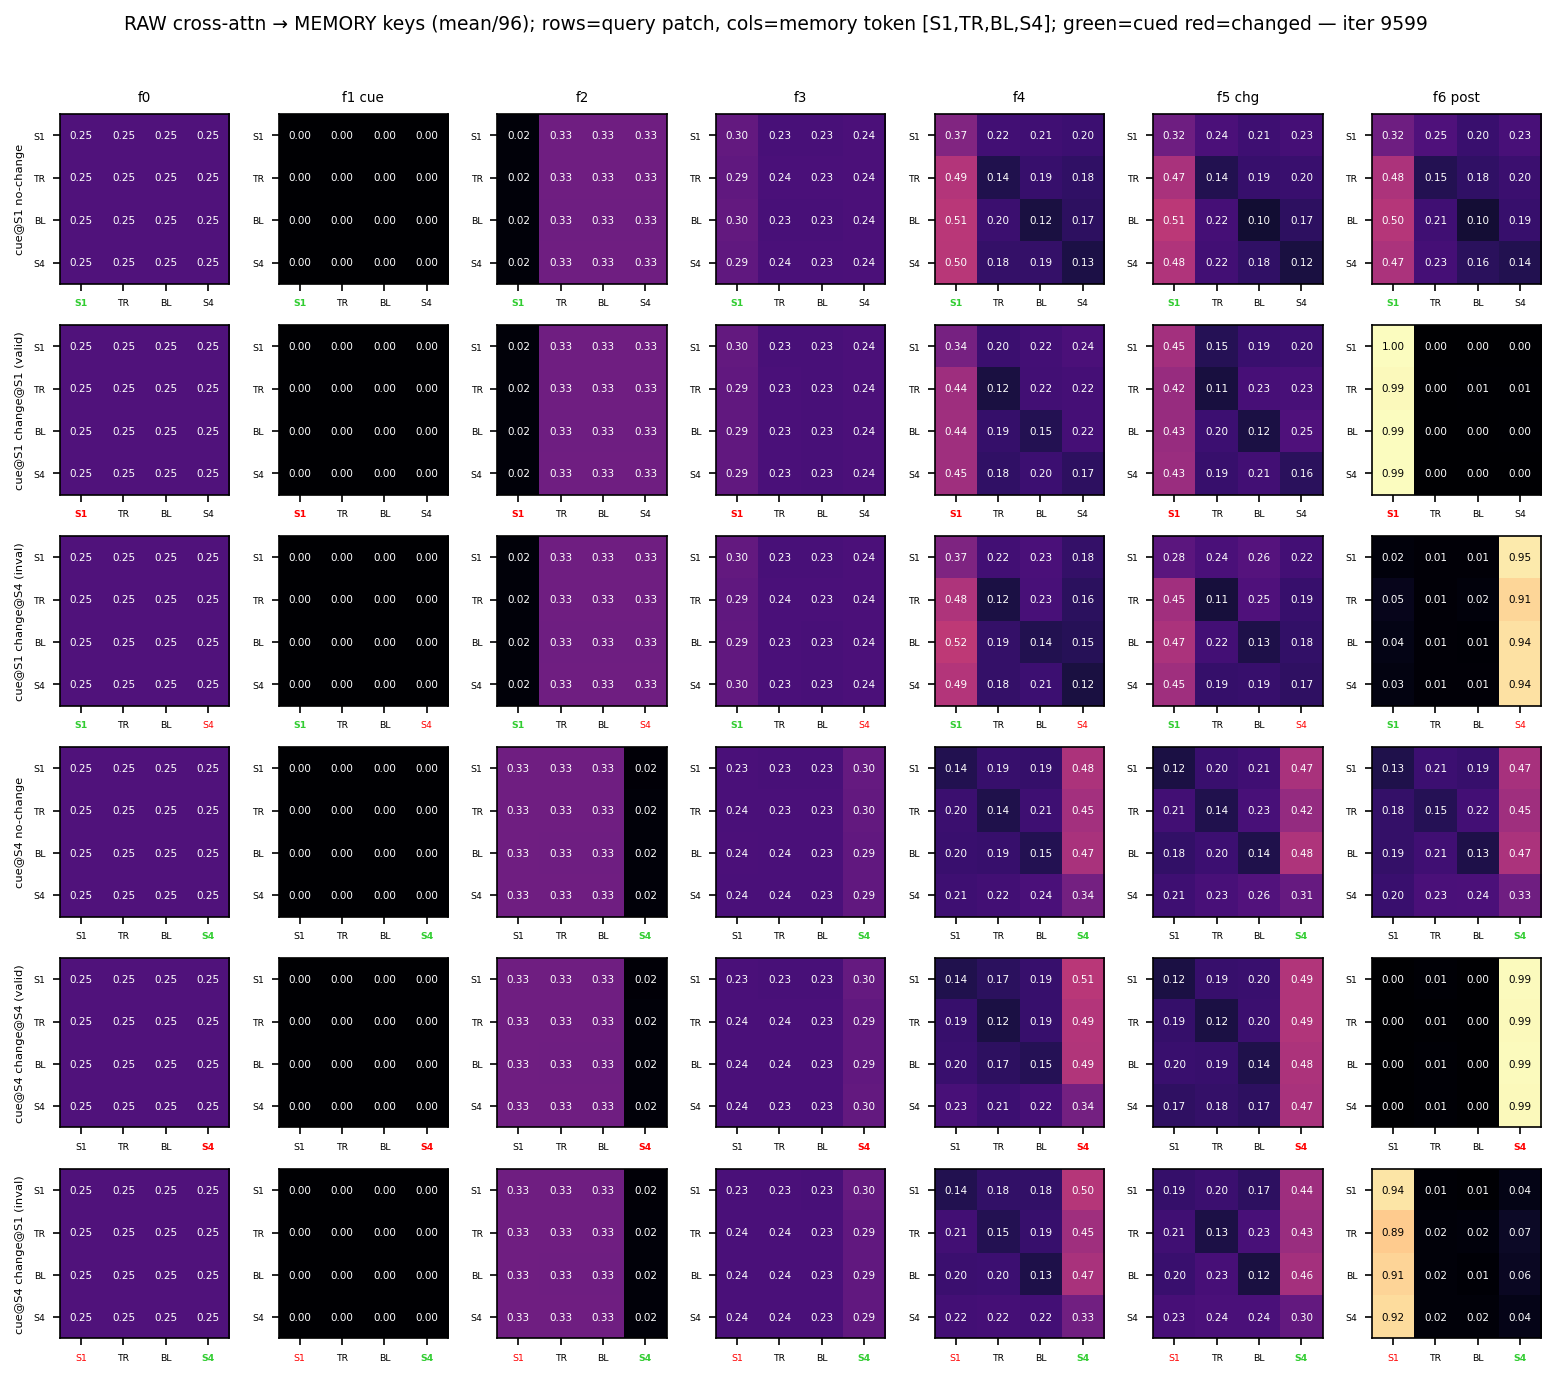
\includegraphics[width=\textwidth]{dd2_maps_memory.png}
\caption{\textbf{Raw memory-key attention maps}, mean over $96$ trials; layout as
Fig.~\ref{fig:mapimg} but columns are memory tokens. The change-lock is the migration of mass onto the
red (changed) column: present at $t{=}5$ for valid changes (rows 2,5), delayed to $t{=}6$ for invalid
changes (rows 3,6).}
\label{fig:mapmem}
\end{figure}

\begin{table}[t]\centering\small
\caption{\textbf{Change-lock timing} (memory-key excess over uniform on the \emph{changed} token, max
over queries). Valid changes lock at $t{=}5$; invalid changes lock only at $t{=}6$.}
\label{tab:lock}
\begin{tabular}{lcc}
\toprule
condition & excess @ $t{=}5$ & excess @ $t{=}6$ \\
\midrule
cue@S1, change@S1 (valid)   & $+0.20$ & $+0.75$ \\
cue@S4, change@S4 (valid)   & $+0.24$ & $+0.74$ \\
cue@S1, change@S4 (invalid) & $-0.03$ & $+0.70$ \\
cue@S4, change@S1 (invalid) & $-0.02$ & $+0.69$ \\
\bottomrule
\end{tabular}
\end{table}

\subsection{Attention allocation is invariant to validity and value}
Sweeping cue validity (proportion $0.25$--$1.0$) and cue value (colour, value $1$--$5$) leaves the
attention maps essentially unchanged (Fig.~\ref{fig:propmet},~\ref{fig:colmet}): the cue-frame read
stays at $\approx\!1.0$ and the change-lock at $\approx\!0.75$ regardless. The model does not grade its
spatial attention by how reliable or how valuable the cue is; it always fully orients to the cued
location. Validity and value therefore act downstream, at the decision (Sec.~4.1), not on the attention
allocation---a dissociation between the \emph{deployment} of attention and its \emph{behavioural use}.

\begin{figure}[t]\centering
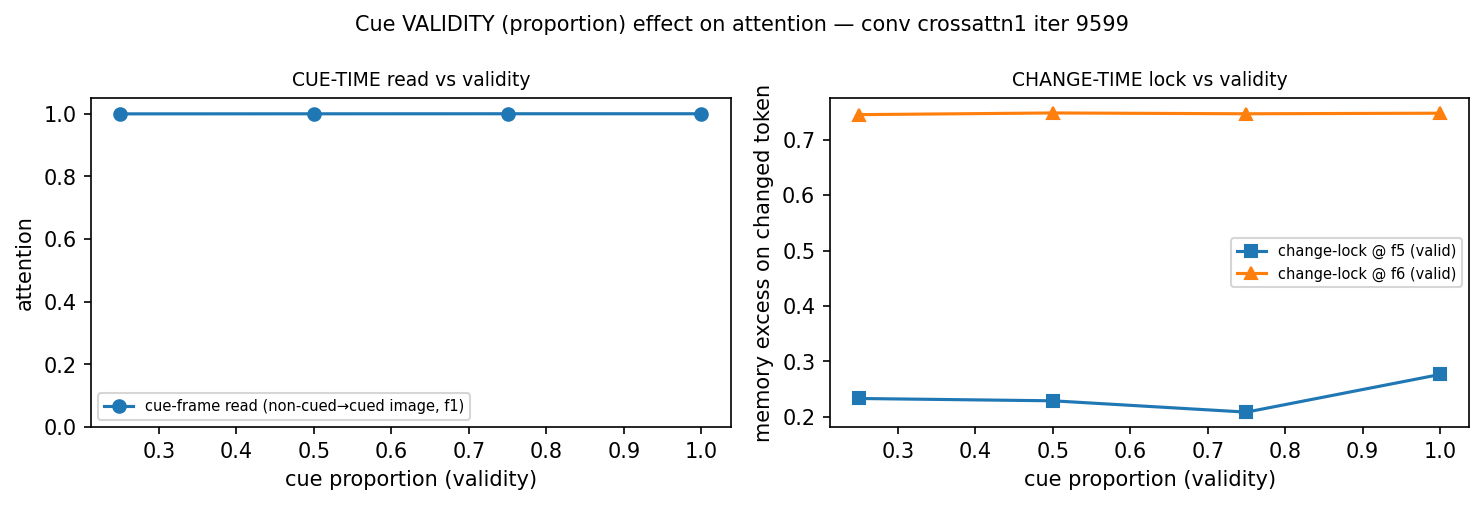
\includegraphics[width=0.92\textwidth]{dd3_proportion_metrics.png}
\caption{\textbf{Validity (proportion) sweep.} Cue-time read (left) and change-time lock (right) vs.\
displayed cue proportion. Both are flat: attention is validity-invariant.}
\label{fig:propmet}
\end{figure}
\begin{figure}[t]\centering
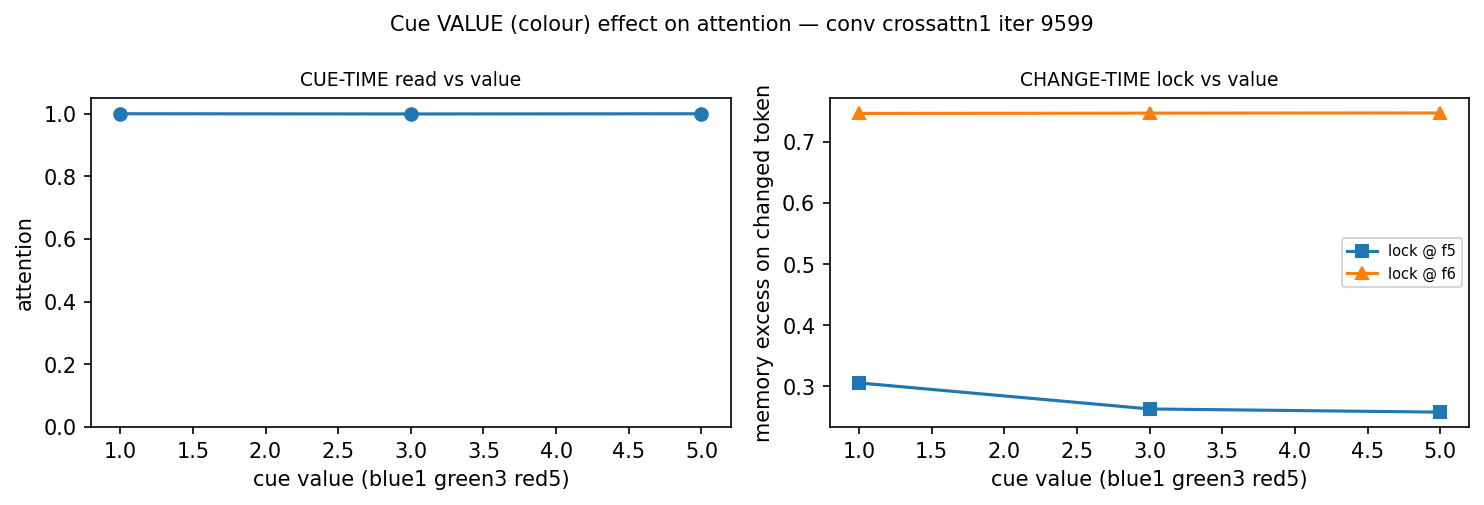
\includegraphics[width=0.92\textwidth]{dd3_colour_metrics.png}
\caption{\textbf{Value (colour) sweep.} Cue-time read and change-time lock vs.\ cue value
(blue$=1$, green$=3$, red$=5$). Both are flat: attention is value-invariant. Memory-key maps at each
proportion/value are shown in the supplement figures \texttt{dd3\_proportion\_maps},
\texttt{dd3\_colour\_maps}.}
\label{fig:colmet}
\end{figure}

\begin{figure}[t]\centering
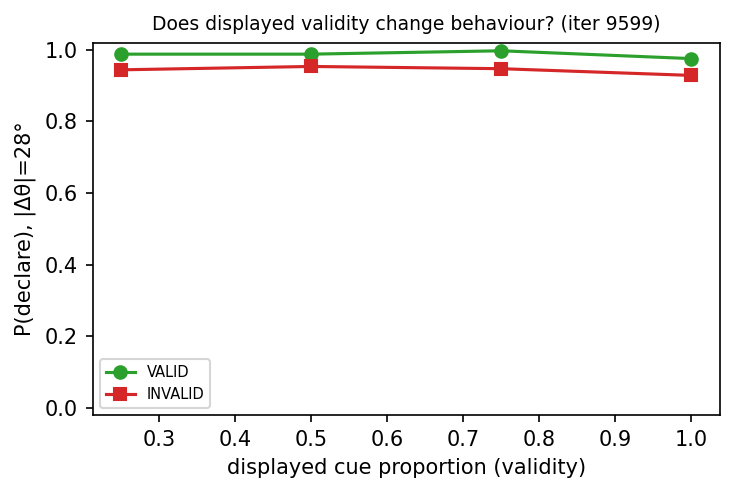
\includegraphics[width=0.55\textwidth]{dd4_validity_behaviour.png}
\caption{\textbf{Displayed validity does not change behaviour.} $P(\text{detect})$ at
$|\Delta\theta|=28^\circ$ for valid vs.\ invalid changes across displayed proportions; the gap is
constant, confirming the cueing benefit is spatial, not a read-out of ring completeness.}
\label{fig:valbeh}
\end{figure}

\subsection{Temporal decoding of the recurrent state}
Linear decoding of $\mathrm{vec}(H^{(t)})$ reveals what the recurrence holds and when
(Fig.~\ref{fig:dec}). Cue position and cue value are decoded \emph{perfectly} ($1.00$, $4$-way and
$3$-way) from the cue frame $t{=}1$ onward and held for the remainder of the trial: the memory latches
both the location and the value of the cue immediately. Strikingly, value is fully present in the
recurrent state even though attention never grades by value (Sec.~4.5)---value resides in memory,
available to the decision, without scaling the attention map. Change presence and change location are at
chance until the change occurs, then rise to $0.88$ and $0.97$ on the change frame $t{=}5$ and to $0.98$
and $0.99$ at $t{=}6$. The change is thus fully localised in the recurrence already at $t{=}5$, one frame
\emph{before} the invalid-condition attention change-lock forms at $t{=}6$ (Table~\ref{tab:lock}): the
recurrence computes the change within the frame and the attention re-points to it on the next frame,
making the ``recurrence computes, attention reflects'' relationship explicit.

\begin{figure}[t]\centering
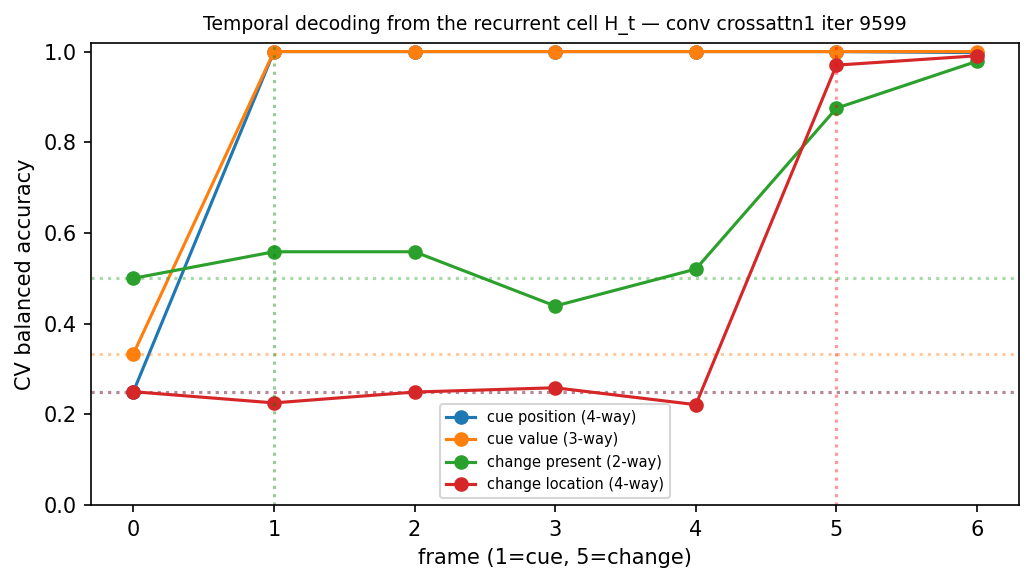
\includegraphics[width=0.72\textwidth]{dd5_decoding.png}
\caption{\textbf{Temporal decoding} (4-fold CV balanced accuracy of logistic regression on the
recurrent cell $H^{(t)}$; dotted lines are chance). Cue position and value are perfectly decodable from
$t{=}1$; change presence/location rise sharply at the change frame $t{=}5$.}
\label{fig:dec}
\end{figure}

\subsection{Causal role of the memory read}
Additively suppressing memory-key attention during the Gabor phase tests whether the change-lock is
necessary for detection (Fig.~\ref{fig:causal}). Suppressing the \emph{cued} quadrant's memory token has
only a small cost (e.g.\ $P(\text{detect})$ at $16^\circ$ falls $0.57\!\to\!0.47$). Suppressing
\emph{all} four memory tokens---forcing the block to read only the current image through attention---
costs more at high magnitude ($0.98\!\to\!0.84$ at $28^\circ$; $0.99\!\to\!0.84$ at $64^\circ$) but does
\emph{not} abolish detection. Detection therefore does not require the memory read: the changed Gabor
enters the cell through the residual $X^{(t)}$ (Sec.~3.2) and is detected there---consistent with the
$t{=}5$ decodability above---while the memory read \emph{refines} the decision by $\sim\!0.1$--$0.15$.
The change-lock is thus partially causal but not the primary carrier of the change signal.

\begin{figure}[t]\centering
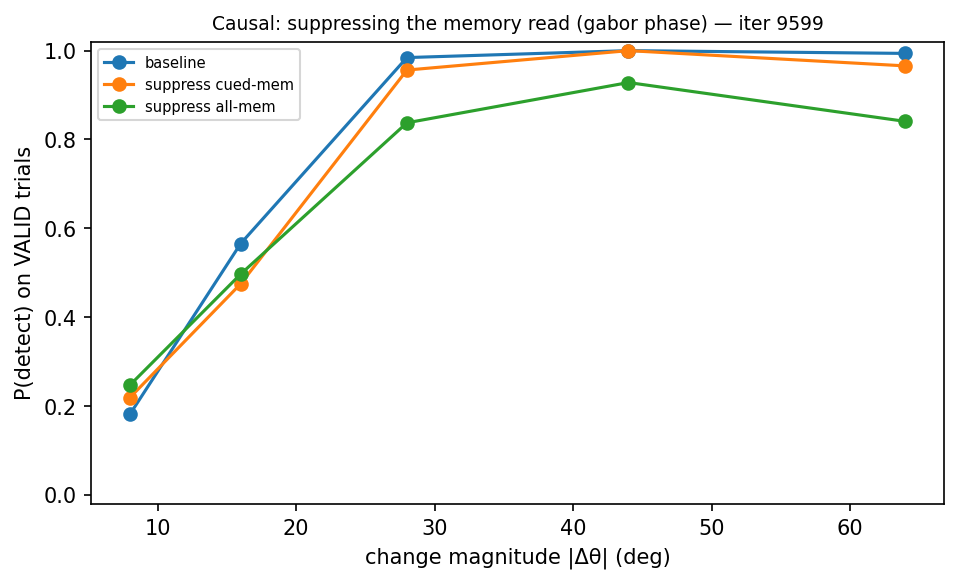
\includegraphics[width=0.6\textwidth]{dd5_causal.png}
\caption{\textbf{Causal perturbation of the memory read} on validly cued trials. Suppressing the cued
memory token (orange) barely changes detection; suppressing all memory tokens (green) costs
$\sim\!0.1$--$0.15$ at high magnitude but detection survives, indicating the change rides in on the
residual image path while the memory read refines the decision.}
\label{fig:causal}
\end{figure}

\section{Discussion}
The trained agent implements a compact, legible attentional algorithm: \emph{orient to the cue once,
encode it, then monitor the cued location from memory and re-point to a change}. Three features make
this a faithful model of covert spatial attention. First, attention is deployed to the cued location
ahead of the target, covertly (no input movement), and the current image continues to drive the cell
through the residual even when image \emph{attention} is withdrawn---separating ``where I attend'' from
``what I can see''. Second, the cue produces a behavioural benefit (lower detection threshold for valid
changes) and an attentional benefit (one-frame-earlier change-lock for valid changes), the two linked by
the same cued-location monitoring. Third, validity and value are integrated at the decision rather than
by scaling the attention map, a specific and testable claim about \emph{where} reliability and reward
enter the computation. In companion analyses of the same architecture family (reported separately), the
cross-attention front-end produces a far sharper, more interpretable allocation than the diffuse,
recurrence-dominated solutions found when the network is trained from raw pixels with held
(frame-repeated) inputs, suggesting that the perceptual front-end and task temporal structure---not the
memory size---determine whether attention or recurrence carries the computation. We next turn to the causal sufficiency of the memory change-lock and to the same battery
across the architecture family.

\end{document}
